\chapter{Hopping frequency}

In the previous chapter we focused on the effective potential obtained by the
superposition of the averaged superposition of the perturbation potential and
the lattice potential. In this chapter we want to emphasize on the physics
that determine the time scale of the perturbation potential.

\section{Harmonic approximation}

Given the effective lattice potential \cref{eq:potential_effective} the
effective lattice Hamiltonian reads
\begin{equation}
  \hat{H}_\text{eff}
  =\frac{\hat{p}^2}{2m}+\hat{V}_\text{eff}
  \label{eq:hamiltonian_effective}.
\end{equation}
One first naive approach to solve the time-independent Schrödinger equation
subject to the effective lattice Hamiltonian would be to Taylor expand
the effective potential in second order
\begin{equation}
  \hat{V}_\text{eff}
  =V_0\cos^2(kx)
  \approx V_0\left(1-\frac{1}{2}(kx)^2\right)
  \label{eq:potential_harmonic_approximation}.
\end{equation}
With \cref{eq:potential_harmonic_approximation} we get the Hamiltonian of a
linear harmonic quantum oscillator
\begin{equation}
  \hat{H}_\text{har}-V_0
  =\frac{\hat{p}^2}{2m}-\frac{1}{2}V_0k^2x^2
  \label{eq:hamiltonian_harmonic_approximation}
\end{equation}
with well-known energy levels
\begin{equation}
  E_n=\hbar\omega(2n+1)/2
  \qc
  \omega=\sqrt{\abs{V_0}/m}k=\sqrt{2\abs{V_0}E_r}/\hbar
  \label{eq:energy_harmonic_approximation}
\end{equation}
where we introduced the recoil energy $E_r=(\hbar k)^2/(2m)$ as an
atom-independent energy scale. In natural scales of the quantum oscillator
we find the time independent wave functions for energy level $n$ to be
\begin{equation}
  \psi_n(x)
  =
  \bra{x}\ket{\psi}
  =
  \frac{\exp(-\frac{1}{2}x^2)}{\sqrt{2^nn!}\pi^{1/4}}H_n(x)
  \label{eq:wavefunction_harmonic}
\end{equation}
where $H_n(x)$ is the $n$th Hermite polynom and the spatial dimension is
expessed in units of $(2E_r/\abs{V_0})^{1/4}/k$.

In \Cref{fig:wavefunction_harmonic} we have visualized the harmonic
approximation for lattice depths $V_0=-50E_r$ including the probability
densities of the wave functions up to the fourth energy level.

\begin{figure}[ht]
  \centering
  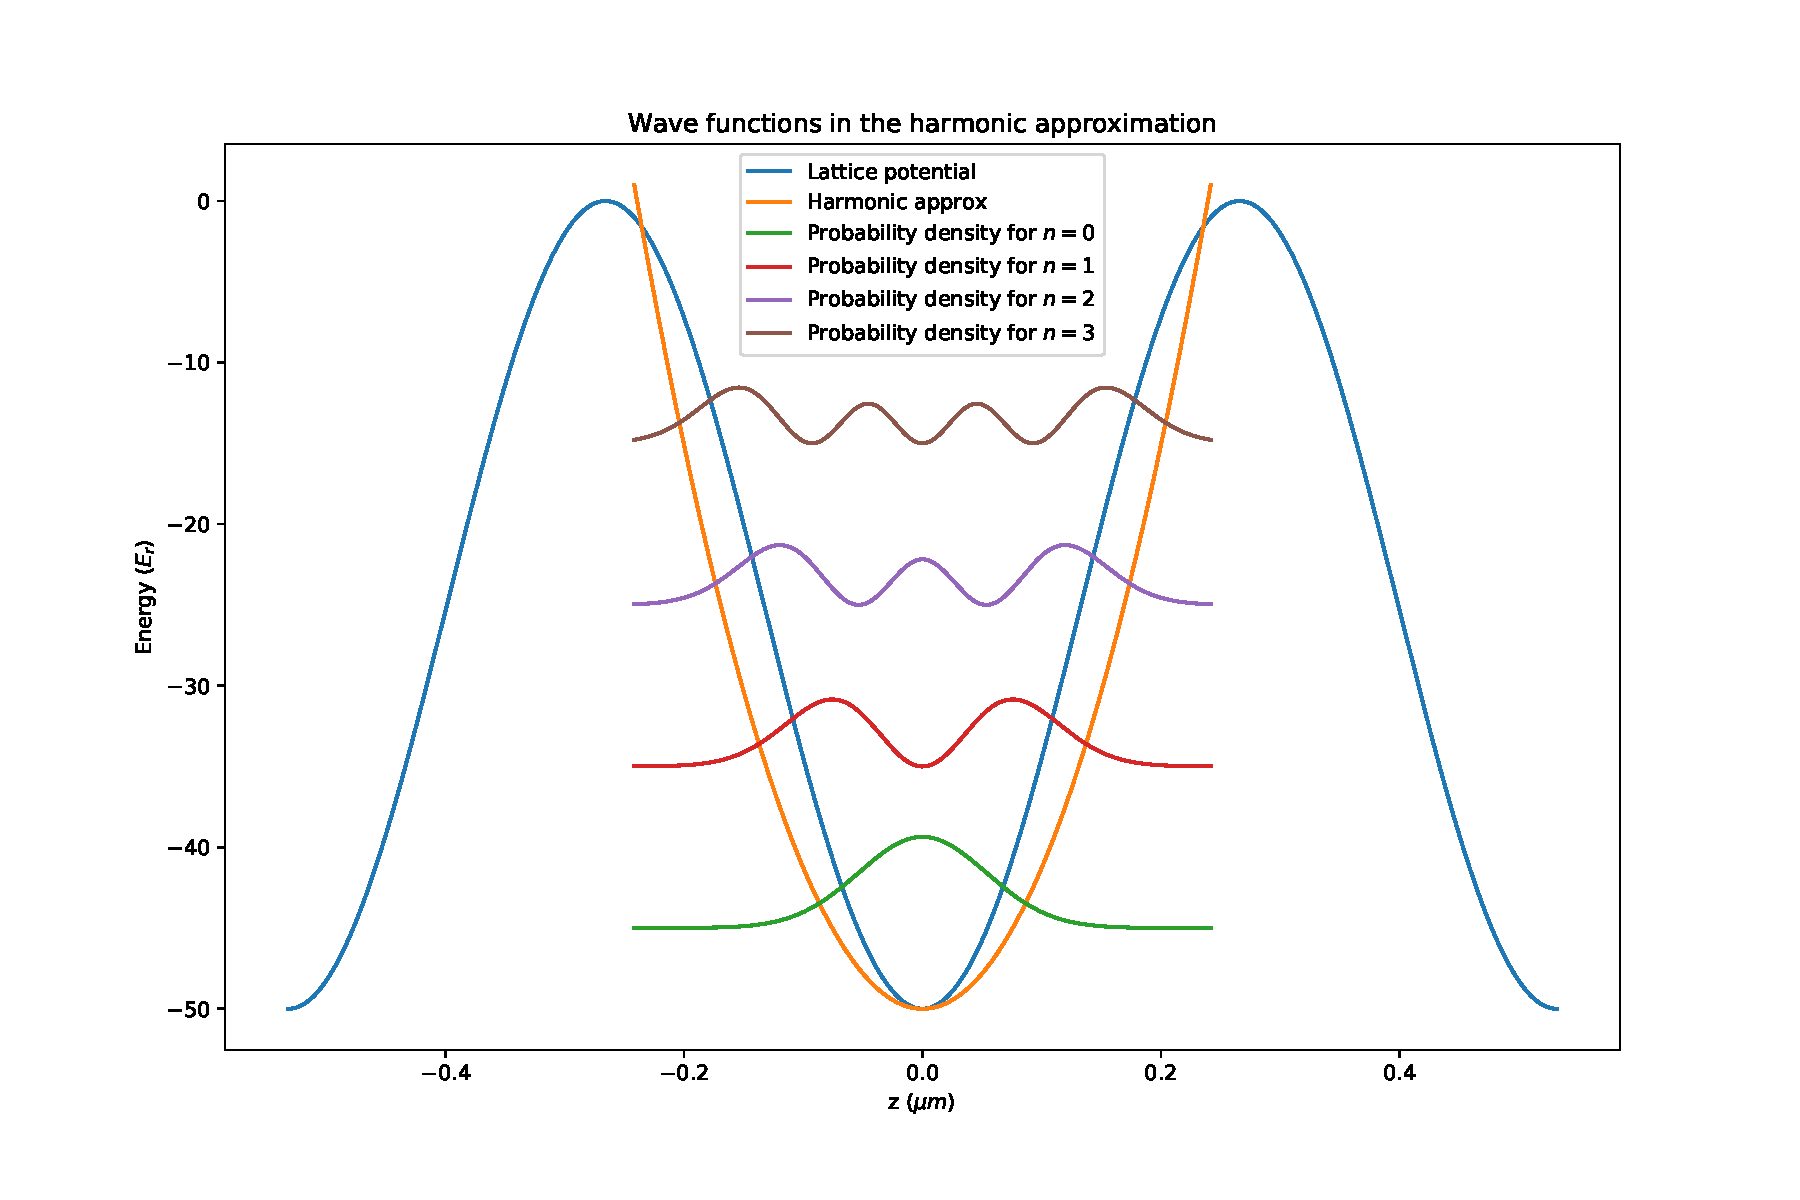
\includegraphics[width=\textwidth]{\figuredir{hopping/harmonic.pdf}}
  \captionsetup{width=.9\textwidth}
  \caption{Harmonic approximation of the optical lattice potential with
    probability density of harmonic wave functions. We can see that the
    probability density decays exponentially at the potential boundaries
    such that the probability for an atom to tunnel to the neighbouring
    lattice site vanish.
  }
  \label{fig:wavefunction_harmonic}
\end{figure}

We can see that the probablity density decays exponentially at the potential
boundary and thereby the probability for a particle to tunnel through the
lattice potential vanishes. We conclude that the harmonic approximation is
not suited to describe the hopping probability and we proceed with a more
elaborate treatment of \cref{eq:hamiltonian_effective} in the next section.

\section{Periodic lattice potentials}

The following section is dedicated to the quantum mechanics of periodic
lattice potentials. We will develope a toolset which allows us to find an
exact solution to \cref{eq:hamiltonian_effective} and other periodic
potentials. We are going to start of with a recap of lattice structures and
examine how Bloch states can be used as ansatz for periodic potentials. From
there on we will derive a general expression for the energy band structure
that arises with Bloch states and then finally discuss Wannier states as
a change of reference frame from the expanded lattice structure to the local
lattice sites.

\subsection{Lattice structures}

A Bravais lattice of dimension $N$ consists of the discrete points
\begin{equation}
  \vb{r}
  =\bra{\vb{x}}\ket{\vb{r}}
  =\sum_{i=1}^Nn_i\vb{a}_i
  \qc n_1,\dots,n_N\in\mathbb{Z}
\end{equation}
where $\vb{a}_i$ are the primitive vectors that span the primitive lattice
cell. We define the reciprocal lattice as the discrete points
\begin{equation}
  \vb{g}
  =\bra{\vb{p}}\ket{\vb{g}}
  =\sum_{i=1}^Nm_i\vb{b}_i
  \qc m_1,\dots,m_N\in\mathbb{Z}
\end{equation}
that satisfy the condition $\exp(\vb{r}\cdot\vb{g})=1$. For a simple cubic
lattice structure $\vb{b}_i=2\pi\vb{a}/{{\vb{a}_i}^2}$ satisfies said
condition. For the subsequent sections we will only consider the one
dimensional simple cubic lattice. Cubic lattices of higher dimension however
can be easily obtained by superposition of the potentials.

As the reciprocal lattice space can be seen as the Fourier transform of the
Bravais lattice, it is especially simple to express periodic functions and it
suggests the representation of periodic potentials in reciprocal lattice
space. Let $\ket{g_n}$ denote the $n$th reciprocal lattice point then the
transformation rule is
\begin{equation}
  \bra{g_n}\hat{V}\ket{g_m}
  =\int\dd{x}\bra{g_n}\ket{x}^*V(x)\bra{g_m}\ket{x}
  =\int\dd{x}V(x)e^{2ikx(n-m)}
  \label{eq:potential_in_reciprocal_lattice}.
\end{equation}
Evaluation of \cref{eq:potential_in_reciprocal_lattice} for a specific
potential will usually yield a finite number of terms in dependence of
$n-m$ as we actually determine the Fourier coefficients of a discrete Fourier
transform.

\subsection{Bloch states}

Bloch's theorem states that for a periodic lattice potential
\begin{equation}
  V_\text{lat}(\vb{x}+\vb{a})=V_\text{lat}(\vb{x})
  \label{eq:potential_periodic}
\end{equation}
there exists a complete set of wavefunctions that are energy eigenstates
of the Hamiltonian
\begin{equation}
  \hat{H}_\text{lat}
  =\frac{\hat{\vb{p}}^2}{2m}+\hat{V}_\text{lat}
  \label{eq:hamiltonian_periodic},
\end{equation}
and each of these Bloch waves can be written into the form
\begin{equation}
  \bra{\vb{x}}\ket{\Psi^n_{\vb{q}}}
  =\Psi^n_{\vb{q}}(\vb{x})
  =e^{i\vb{q}\cdot\vb{x}}\psi^n_{\vb{q}}(\vb{x})
  \label{eq:state_bloch}
\end{equation}
with $\psi^n_{\vb{q}}(\vb{x}+\vb{a})=\psi^n_{\vb{q}}(\vb{x})$, wave vector
$\vb{q}$ and bandindex $n$. We confine the wave number to the first Brillouin
zone $-k<q<+k$. For a proof of Bloch's theorem see \cite{Roessler2004} or
\cite{Bartelmann2018}.

\subsection{Energy bands}

The Bloch states \cref{eq:state_bloch} can be used as ansatz to solve the
periodic lattice Hamiltonian
\begin{equation}
  \hat{H}_\text{lat}
  =\frac{\hat{p}^2}{2m}+\hat{V}_\text{lat}
  \label{eq:hamiltonian_lattice}.
\end{equation}
We notice that by the product rule
$\hat{p}^2\Psi^n_q(x)=e^{iqx}(\hat{p}+\hbar q)\psi^n_q(x)$,
thus we find
\begin{equation}
  E^n_q\ket{\Psi^n_{q}}
  =\hat{H}_{lat}\ket{\Psi^n_{q}}
  =e^{iqx}\left(\frac{(\hat{p}+\hbar q)^2}{2m}+\hat{V}_\text{lat}\right)\ket{\psi^n_{q}}
  \label{eq:eigenvalue_energy_lattice}.
\end{equation}
Expansion of the state $\ket{n,q}$ in states of the reciprocal lattice returns
\begin{equation}
  \ket{\Psi^n_q}
  =\left(\sum_s\ket{g_s}\bra{g_s}\right)\ket{\Psi^n_q}
  =\sum_s\braket{g_s}{\Psi^n_q}\ket{g_s}
  =\sum_sc^n_{sq}\ket{g_s}
  \label{eq:state_bloch_in_reciprocal_lattice}.
\end{equation}
The momentum eigenvalues of the state $\ket{g_s}$ can be found by expansion
into position space
\begin{equation}
  \hat{p}\ket{g_s}
  =\int\int\dd{x}\dd{y}\ket{y}\bra{y}\hat{p}\ket{x}\bra{x}\ket{g_s}
  \label{eq:eigenvalue_momentum_reciprocal_lattice1}.
\end{equation}
With $\bra{y}\hat{p}\ket{x}=-i\hbar\delta(y-x)\dv{x}$ we can take the
derivative of $\bra{x}\ket{g_s}=e^{2ikxs}$ and simplify
\cref{eq:eigenvalue_momentum_reciprocal_lattice1} down to
\begin{equation}
  \hat{p}\ket{g_s}
  =2\hbar ks\int\dd{x}\ket{x}\bra{x}\ket{g_s}
  =2\hbar ks\ket{g_s}
  \label{eq:eigenvalue_momentum_reciprocal_lattice2}.
\end{equation}
Finally we insert \cref{eq:state_bloch_in_reciprocal_lattice} into
\cref{eq:eigenvalue_energy_lattice} and apply $\bra{g_t}$ to the
right hand side while using \cref{eq:potential_in_reciprocal_lattice} and
\cref{eq:eigenvalue_momentum_reciprocal_lattice2}, yielding
\begin{equation}
  E^n_qc^n_{tq}
  =c^n_{tq}\frac{(2s+q/k)^2}{2m}E_r+\sum_sc^n_{sq}\bra{g_t}\hat{V}_\text{lat}\ket{g_s}
  \label{eq:eigenvalue_energy_lattice_explicit}
\end{equation}
with recoil energy $E_r=\hbar^2k^2/(2m)$.
\Cref{eq:eigenvalue_energy_lattice_explicit} has to be solved for known
$\hat{V}_\text{lat}$ numerically. We will do this later for the effective
optical lattice potential from \cref{eq:potential_effective}.

\subsection{Wannier states}

So far we studied the effects of a periodic lattice potential on the energy
levels and the Bloch wave functions that propagate over the complete lattice.
Lattice hopping however is a local effect, therefore we need a spatially
localized set of wave functions to describe the effect of lattice hopping.
Fortunately the so called Wannier fullfill these requirements.

\subsubsection{Definition via Bloch superpositions}

The orthodox definition of the Wannier function with bandindex $n$ at lattice
site $l$ reads
\begin{equation}
  \ket{\phi^n_{l}}
  =\frac{1}{\sqrt{N}}\sum_qe^{-iqla}\ket{\Psi^n_{q}}
  \label{eq:state_wannier_orthodox}
\end{equation}
wherein $\ket{\Psi^n_q}$ is the Bloch wave functions from
\cref{eq:state_bloch}, $N$ the total number of lattice sites and the sum
over $q$ is confined to the first Brillouin zone with $q$ that satisfy the
periodic boundary condition $-k<q=2ki/N<+k$ with integer $i\in\mathbb{Z}$.

\subsubsection{Definition via the band projected position operator}

The defintion \cref{eq:state_wannier_orthodox} is valid for simple lattice
structures, however for more sophisticated lattices Gauge freedom of the
phase of the Bloch states leads to different Wannier states, whereof only
one is the maximally localized one \cite{Goerg2014}. One can find the
phase of the Bloch state that is maximally localized by minimizing the spread
of the Wannier states, however there also exists a more general definition
that incorporates the phase ubiquity. In the general definition the Wannier
states are best to construct as the eigenstates of the band projected
position operator. The band projector to bandindex $n$ is defined as
\begin{equation}
  \hat{P}_n
  =\sum_q\ket{\Psi^n_q}\bra{\Psi^n_q}
  \label{eq:operator_band_projector}
\end{equation}
and the band projected position operator just follows as
\begin{equation}
  \hat{x}_n
  =\hat{P}_n\hat{x}_n\hat{P}_n
  \label{eq:operator_band_projected_position}.
\end{equation}
The wannier states are now defined as the eigenstates of the eigenvalue
equation
\begin{equation}
  \hat{x}_n\ket{\phi^n_l}=x^n_l\ket{\phi^n_l}
  \label{eq:eigenvalue_band_projected_position}
\end{equation}
where $x^n_l$ is the $l$th lattice site in the $n$th energy band. Choosing
the Bloch base to find the elements of the band projected position operator
\cref{eq:operator_band_projected_position} through
\begin{equation}
  X^{nn^\prime}_{qq^\prime}
  =\bra{\Psi^n_q}\hat{x}_n\ket{\Psi^{n^\prime}_{q^\prime}}
  =\int_0^{Na}\dd{x}\Psi^n_q(x)^*x\Psi^{n^\prime}_{q^\prime}(x)
  \label{eq:element_band_projected_position}
\end{equation}
which give an analytical expression to solve to determine the matrix elements
\cite{Bissbort2013}. Let $d^{mn}_{lq}$ be the diagonalized
matrix $X^{nn^\prime}_{qq^\prime}$ in
\cref{eq:element_band_projected_position} then the Wannier states are fully
determined by
\begin{equation}
  \ket{\phi^n_l}
  =\sum_{n,q}d^{mn}_{lq}\ket{\Phi^n_q}
  \label{eq:state_wannier}.
\end{equation}

\subsection{Hopping amplitude}

With the previous tools in place we are now set to give an expression for the
quantum hopping amplitude between lattices.

We define the hopping probability from lattice site $l$ to lattice site
$l^\prime$ at bandindex $n$ as
\begin{equation}
  J^n_{ll^\prime}
  =-\bra{\phi^n_l}\hat{H}_\text{lat}\ket{\phi^n_{l^\prime}}
  \label{eq:element_hopping}
\end{equation}
this definition makes intuitive sense if we remind us at the dipole transition
element and the Wannier states. Using the orthodox definition of the Wannier
states \cref{eq:state_wannier_orthodox} for \cref{eq:element_hopping} we find
\begin{equation}
  J^n_{ll^\prime}
  =\frac{1}{N}\sum_{q,q^\prime}e^{iqa(l-l^\prime)}
  \bra{\Psi^n_q}\hat{H}_\text{lat}\ket{\Psi^n_{q^\prime}}
  \label{eq:element_hopping2}.
\end{equation}
The Bloch states are energy eigenstates
\cref{eq:eigenvalue_energy_lattice_explicit} and orthonormal, henceforth
\begin{equation}
  J^n_{ll^\prime}
  =\frac{1}{N}\sum_{q}E^n_qe^{iqa(l-l^\prime)}
  \label{eq:element_hopping3}.
\end{equation}
Expression \cref{eq:element_hopping3} is exact for a given number of lattices
$N$ and can be evaluated numerically. The form of \cref{eq:element_hopping3}
resembles a discrete Fourier transform. The inverse Fourier transform gives us
the energies in terms of the hopping probabilites
\begin{equation}
  E^n_q
  =\sum_{l-l^\prime}J^n_{l,l^\prime}e^{-iqa(l-l^\prime)}
  \label{eq:element_energy_hopping}
\end{equation}
which in practice is easier to calculate then \cref{eq:element_hopping} as
can be seen in the consecutive section.

\subsubsection{Tight-binding approximation}

For deep potentials $V_0\gtrapprox3E_r$ hopping only contributes from direct
neighbour sites \cite{Rom2009}. Thus we can \cref{eq:element_energy_hopping}
reduces to
\begin{equation}
  E^n_q
  \approx J^n_{l,l+1}e^{-iqa}+J^n_{l,l-1}e^{+iqa}+J^n_{ll}
  =J^n_0+2J^n_1\cos(qa)
  \label{eq:element_energy_hopping_tb_approx}
\end{equation}
where we have $J^n_{l,l-1}=J^n_{l,l+1}=J_1$ because of translation invariance.
Using evaluation of $J^n_0=J^n_{ll}$ with \cref{eq:element_hopping} tells us
that $J^n_0$ just is the average energy of an energy band. Evaluation of
\cref{eq:element_energy_hopping_tb_approx} at $q=0$ and $q=k$ and subtracting
the results from another yields us
\begin{equation}
  J^n_1\approx\frac{1}{4}\left(E^n_k-E^n_0\right)
  \label{eq:hopping_amplitude_energies}
\end{equation}
which says that the hopping probability is approximate one quarter of the
energy bandwidth.

\section{Numerical determination of hopping frequency}

Finally we want to apply the previous results on the previously found
effective potential $V(z)=V_0\cos^2(kz)$ \cref{eq:potential_effective}. Using
\cref{eq:potential_in_reciprocal_lattice} we find that the matrix elements of
the effective potential indeed have the simple form
\begin{equation}
  \bra{g_s}\hat{V}_\text{eff}\ket{g_t}
  =\frac{1}{4}V_0\left(2\delta^s_t+\delta^s_{t-1}+\delta^s_{t+1}\right)
  \label{eq:elements_effective_potential_in_reciprocal_state}
\end{equation}
in reciprocal space. Using
\cref{eq:elements_effective_potential_in_reciprocal_state} for the matrix
elements of the effective Hamiltonian using
\cref{eq:eigenvalue_energy_lattice_explicit} gives us
\begin{equation}
  H_{st}
  =\bra{g_s}\hat{H}_\text{eff}\ket{g_t}
  =\begin{cases}
    (2s+q/k)^2E_r+\frac{1}{2}V_0, & \text{if }s=t\\
    \frac{1}{4}V_0, & \text{if } \abs{s-t}=1\\
    0, & \text{otherwise}
  \end{cases}
  \label{eq:hamiltonian_effective_elements}.
\end{equation}
Now that we have found a definite expression for the Hamiltonian matrix
elements \cref{eq:hamiltonian_effective_elements} we can use the energy
eigenvalue equation \cref{eq:eigenvalue_energy_lattice_explicit} to calculate
the energy bands in dependence of the quasi-momentum $\hbar q$.

\begin{figure}[ht]
  \centering
  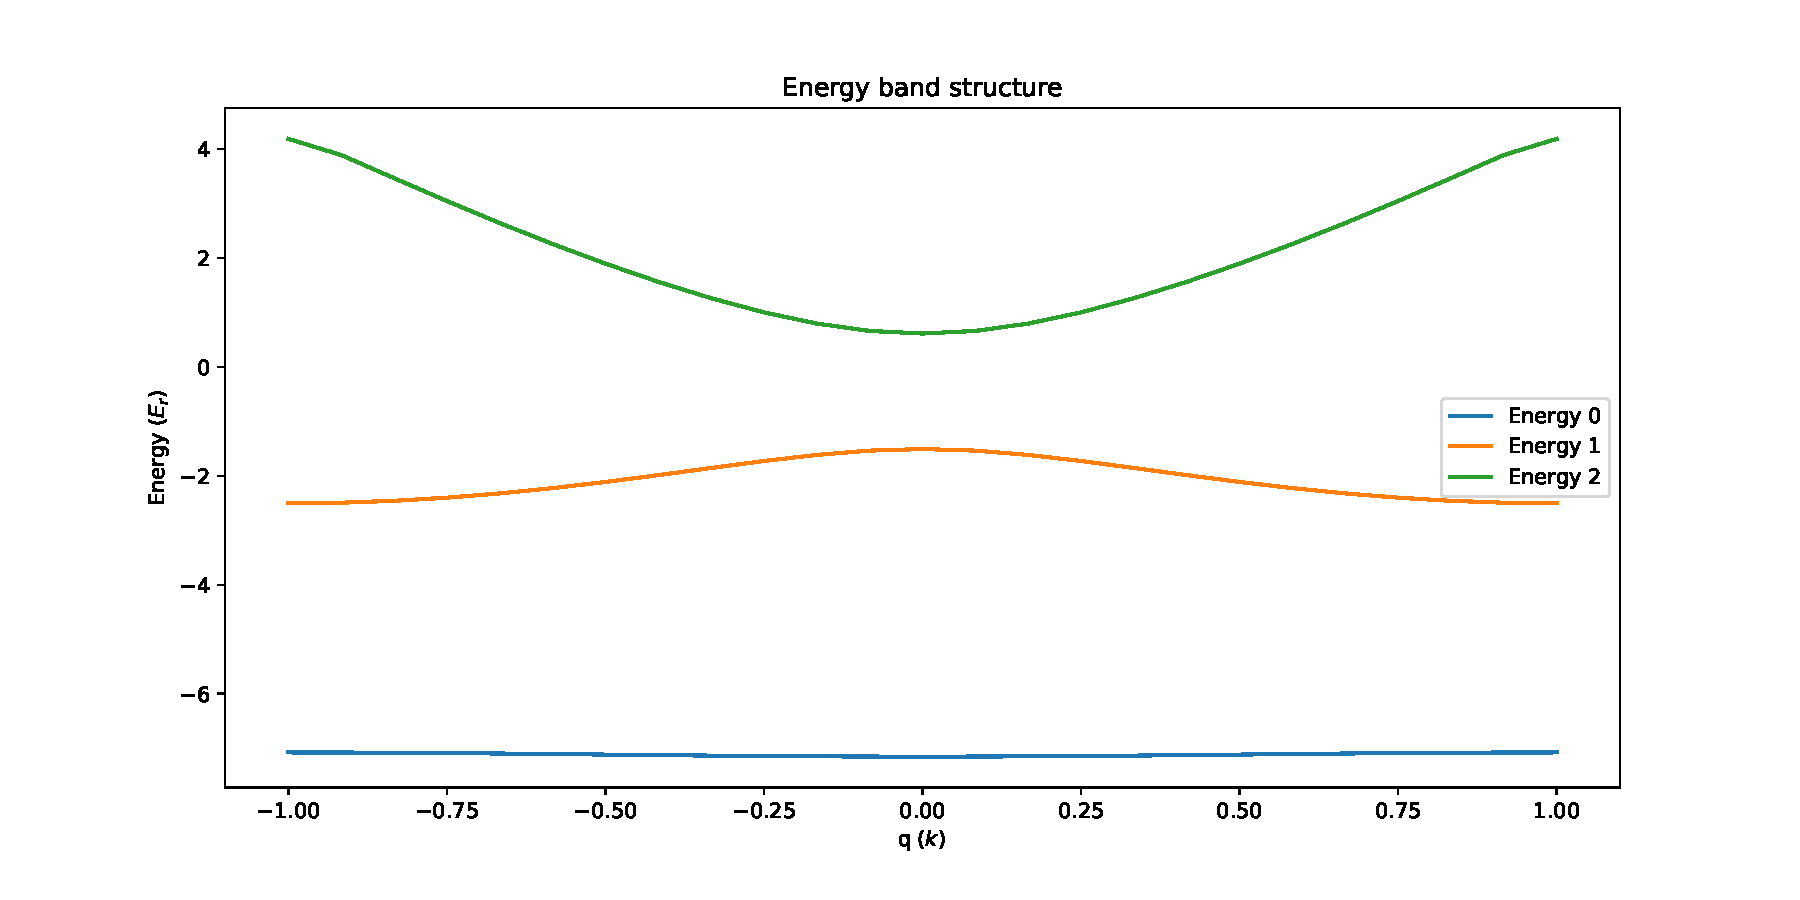
\includegraphics[width=\textwidth]{\figuredir{hopping/band-structure.pdf}}
  \captionsetup{width=.9\textwidth}
  \caption{
    First three energy bands for an optical lattice depth of $V_0=-10E_r$.
  }
  \label{fig:band_structure}
\end{figure}

In \Cref{fig:band_structure} we visualized the first energy bands for a
lattice depth of $V_0=-10E_r$ from a matrix with dimensions 60.

the coefficients of the Bloch states
\cref{eq:state_bloch_in_reciprocal_lattice} numerically and thereof the
hopping terms using either the exact expression
\cref{eq:element_energy_hopping} over all quasi-momenta $\hbar q$ or through
the tight binding approximation \cref{eq:hopping_amplitude_energies}.

\subsection{Analytical proximity}

The literature \cite{Bloch2008} also reports the analytical proxmity
\begin{equation}
  J^n_1\approx
  \frac{4}{\sqrt{\pi}}\left(\frac{V_0}{E_r}\right)^{3/4}\exp(-2\sqrt{V_0/E_r})
  \label{eq:hopping_proximity}
\end{equation}
to be valid for sinusoidal potentials like \cref{eq:potential_effective} and
to be derived from the Mathieu equation. The Mathieu equation can be obtained
from the time-independent Schrödinger equation with
$V_0\cos^2(kx)=\frac{1}{2}V_0\left(1-\cos(2kx)\right)$. \cite{Connor1984}
gives a more elaborate deviation of \cref{eq:hopping_proximity}.

\subsection{Results}

Comparison of different methods to obtain the hopping amplitude and how
they behave for different potential deeps. Conversion of the hopping term to
a frequency and significance for our experiment.
